\documentclass[varwidth=true, border=2pt]{standalone}

\usepackage{pgfplots}
\usepackage{tikz}

\usetikzlibrary{calc,patterns,angles,quotes}

\begin{document}
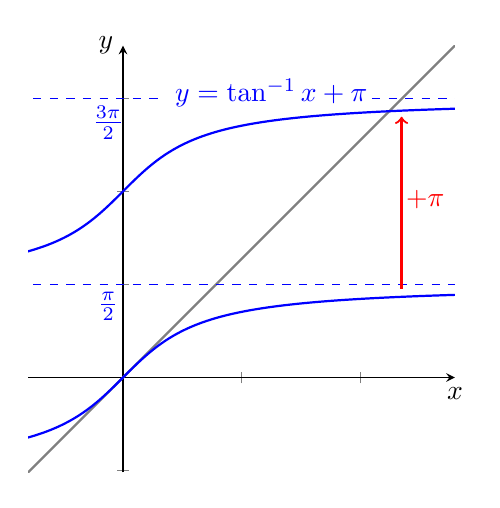
\begin{tikzpicture}
    \begin{axis}[
        legend pos=south east,
        axis x line=middle,
        axis y line=middle,
	every axis x label/.style={at={(current axis.right of origin)},anchor=north},
	every axis y label/.style={at={(current axis.above origin)},anchor=east},
	xticklabels=\empty,
	ytick = {-1.570796, 0, ..., 6.283185},
	yticklabels=\empty,
        grid = none ,
        width=7cm,
        height=7cm,
        grid style={dashed, gray!1},
        xmin=-1,     % start the diagram at this x-coordinate
        xmax= 5,    % end   the diagram at this x-coordinate
        ymin=-1,     % start the diagram at this y-coordinate
        ymax=5,   % end   the diagram at this y-coordinate
        xlabel=$x$,
        ylabel=$y$,
        enlargelimits=true,
        tension=0.08]

         \addplot[domain=-5:6, gray, thick,samples=250] {x};
        \addplot[domain=-5:6,blue, thick,samples=250] {rad(atan(x))};
        \addplot[domain=-5:6,blue, thick,samples=250] {rad(atan(x))+3.14159};

	\draw[blue, dashed](axis cs: -6,1.5708)--(axis cs: 6,1.5708);
	\draw[blue, dashed](axis cs: -6,4.71239)--(axis cs: 0.7,4.71239);
	\draw[blue, dashed](axis cs: 4.2,4.71239)--(axis cs: 6,4.71239);
	\draw[red, thick, ->](axis cs: 4.7,1.5)--(axis cs: 4.7, 4.4);
%	\draw[red, dashed](axis cs: -4.7124, -6)--(axis cs: -4.7124, 6);
%	\draw[red, dashed](axis cs: 4.7124, -6)--(axis cs: 4.7124, 6);
	
	\node[red] (A1) at (axis cs: 5.1,3){$+\pi$};
	\node[blue] (A2) at (axis cs: 2.5,4.8){$y = \tan^{-1} x + \pi$};
	\node[blue] (A3) at (axis cs: -0.25,1.2){$\frac{\pi}{2}$};
	\node[blue] (A4) at (axis cs: -0.25,4.3){$\frac{3 \pi}{2}$};
    \end{axis}
\end{tikzpicture}
\end{document}